\section{Das McCulloch-Pitts-Neuron}\label{sec:mcpneuron}

Im Jahr 1943 veröffentlichen \textit{Warren McCulloch} und \textit{Walter Pitts}\footnote{
    siehe Anhang~\ref{appendix:mcculloch}
} ihre Arbeit~\cite{MP43}.
Sie stellen darin ein auf \textbf{Aussagenlogik}\footnote{
    Die (zweiwertige) Aussagenlogik beschäftigt sich mit der Verknüpfung von Aussagen und deren Wertigkeit unter der Berücksichtigung der Wahrheitswerte ``wahr`` und ``falsch`` (vgl.~\cite[2]{Rau88}).
} basierendes mathematisches Modell zur Erklärung von Signalverarbeitung und  -weiterleitung im Nervensystem vor, und liefern damit grundlegende Ideen für die Kybernetik\footnote{
    siehe Anhang~\ref{appendix:wiener}
} und die Von-Neumann-Rechnerarchitektur\footnote{
    Die Architektur zeichnet sich durch eine Zentraleinheit, der Speichereinheit und Ein-/Ausgabeinheit aus, die über Busse verbunden sind (vgl.~\cite[230]{OV00})
}. Insgesamt leisten sie damit einen wichtigen Beitrag für die Entwicklung \textit{Künstlicher Intelligenz}(vgl.~\cite[1]{Arb19}).


\subsection{Der Kalkül}

In der \textbf{Principia Mathematica}\footnote{
    Die \textbf{Principia Mathematica}~\cite{PW27} (PM) der Philosophen und Mathematiker Bertrand Russell (1872 - 1970) und Alfred Whitehead (1861 - 1947) ist ein Werk über die Grundlagen der Mathematik und erschien in drei Bänden zwischen 1910 und 1913.
} stellen \textit{Russel} und \textit{Bertrand} die Mathematik auf ein Gerüst logischer Grundprinzipien (vgl.~\cite[225]{She26}). Inspiriert dadurch beschäftigt sich McCulloch mit der Frage, ob es nicht auch möglich sei, die Vorgänge im Gehirn durch Anwendung logischer Prinzipien erklärbar zu machen (vgl.~\cite[4]{Arb19}). Die Zweiwertigkeit des Alles-oder-nichts-Prinzips (siehe Abschnitt~\ref{sec:aktionspotenzial}) führt zu dem Kalkül:\\

\blockquote[{\cite[100]{MP43}}]{
    The `all-or-none law` of nervous activity is sufficient to insure that the activity of any neuron may be represented as a proposition.
}\\

McCulloch und Pitts gehen für ihren Kalkül von folgenden physischen Eigenschaften einer Nervenzelle aus\footnote{
    Für ihren Kalkül entwerfen sie zwei Netze: Ein zyklenfreies Netz (vgl.~\cite[101]{MP43}) sowie ein Netz, in dem Zyklen vorhanden sind (vgl. ~\cite[108]{MP43}), wobei
    die Frage nach Ursprung und Bedeutung von ``loops`` - also Zyklen - in einem Netz von Nervenzellen McCulloch bereits seit 1928 beschäftigt: ``The tremors of Parkinson’s disease, McCulloch thought, could be explained by closed loops of activity connecting the spinal cord and the contracting muscles.``~\cite[178]{Pic04}. \textit{Arbib} vermerkt in~\cite[3]{Arb19}: ``As another stage in McCulloch's search for the logic of the nervous system, he began thinking about loops in the nervous system. [...] an idea that today we take for granted.`` \textit{Arbib} verweist auf \textit{Lawrence Kubie}, der im Jahr 1930~\cite{Kub30} veröffentlicht, eine Arbeit über ``the possible importance of reverberating loops``~\cite[5]{Arb19}, die für die Forschungen McCullochs wichtig gewesen ist (vgl. ~\cite[5]{Arb19})
} (vgl.~\cite[101]{MP43}):


\begin{enumerate}
    \item Ein Neuron arbeitet auf Basis des Alles-oder-Nichts-Prinzip
    \item Eine gewisse Anzahl von Synapsen muss innerhalb einer bestimmten Zeit angeregt werden, um ein Neuron zu erregen
    \item Die einzige signifikante Verzögerung bei der Signalübertragung innerhalb des Nervensystems ist bedingt durch synaptische Verzögerungen
    \item Eine einzige hemmende Synapse verhindert die Erregung des betreffenden Neurons
    \item Die Struktur des neuronalen Netzes ändert sich nicht
\end{enumerate}


\subsection{Anwendung des Modells}

Im folgenden wollen wir das Modell von McCulloch und Pitts anwenden.
Hierzu überführen wir die für die Original-Arbeit aus der PM entnommene Notation für Aussagenlogik\footnote{
    Die übernommene Notation gilt als sperrig~\cite[16]{AR88}. Eine ausführliche Übersicht der in der PM gebräuchlichen Notation findet sich unter \url{https://plato.stanford.edu/entries/pm-notation/} (abgerufen 10.8.2023)
} in eine geläufigere Form: Wir nutzen ``$\land$`` für \textit{Konjunktion}, ``$\lor$`` für \textit{Disjunktion} sowie ``$\neg$`` für die \textit{Negation}.
``$\equiv$`` verwenden wir im Sinne der Äquivalenz.
Für ``McCulloch-Pitts-Neuron`` verwenden wir im Folgenden abkürzend \textbf{MCP-Zelle}; für ein Netz, das aus MCP-Zellen besteht, einfach \textbf{MCP-Netz}.\\

In Anlehnung an das Original legen wir folgende Anforderungen für die Anwendung fest\footnote{
    vgl.~\cite[26 f.]{Fau94}. Für unsere einführende Betrachtung folgen wir~\cite[33 f.]{Roj93} und ignorieren zunächst die Zeitwerte aus der Original-Arbeit: Dort wird für die Signalübertragung ein diskreter Zeitwert $t \in \mathbb{Z}$ vereinbart: Die Übertragung eines Signals dauert eine Zeiteinheit, also $t + 1$. Vgl. hierzu Abbildung~\ref{fig-mcpcell}.
}
\begin{enumerate}
    \item Das Verhalten des künstlichen Neurons ist zweiwertig, also \textit{binär}. Das Neuron feuert, oder es feuert nicht. Im Sinne der Beziehung zwischen Eingabe und Ausgabe verstehen wir unter ``feuern`` den Wert $1$. Wenn ein Neuron nicht feuert, wird dies durch den Wert $0$ repräsentiert, der ebenfalls als Ausgabe vorliegt. In diesem Sinne produziert unser Modell also immer ein ``Signal``\footnote{
        Die ausbleibende Exoztyose in chemischen Synapsen kann in dem Sinne einer Modellierung als ``0``-Signal verstanden werden (siehe Kapitel~\ref{synaptischeuebertragung}).
    }.
    \item An einem Neuron liegen (beliebig viele) Eingaben an.
    \item Jedes Neuron hat einen individuellen Schwellenwert. Der Schwellenwert muss getroffen oder übertroffen werden, damit das Neuron ``1`` feuert.
    \item Hemmung ist ``absolut``: Liegt ein hemmendes Signal zusammen mit nicht-hemmenden Signalen an, feuert das Neuron nicht\footnote{
        Für eine weitere Ausführung absoluter und relativer Hemmung siehe~\cite[42 f.]{Roj93}.
    }
\end{enumerate}


\begin{figure}[h]
    \label{fig-mcpcell}
    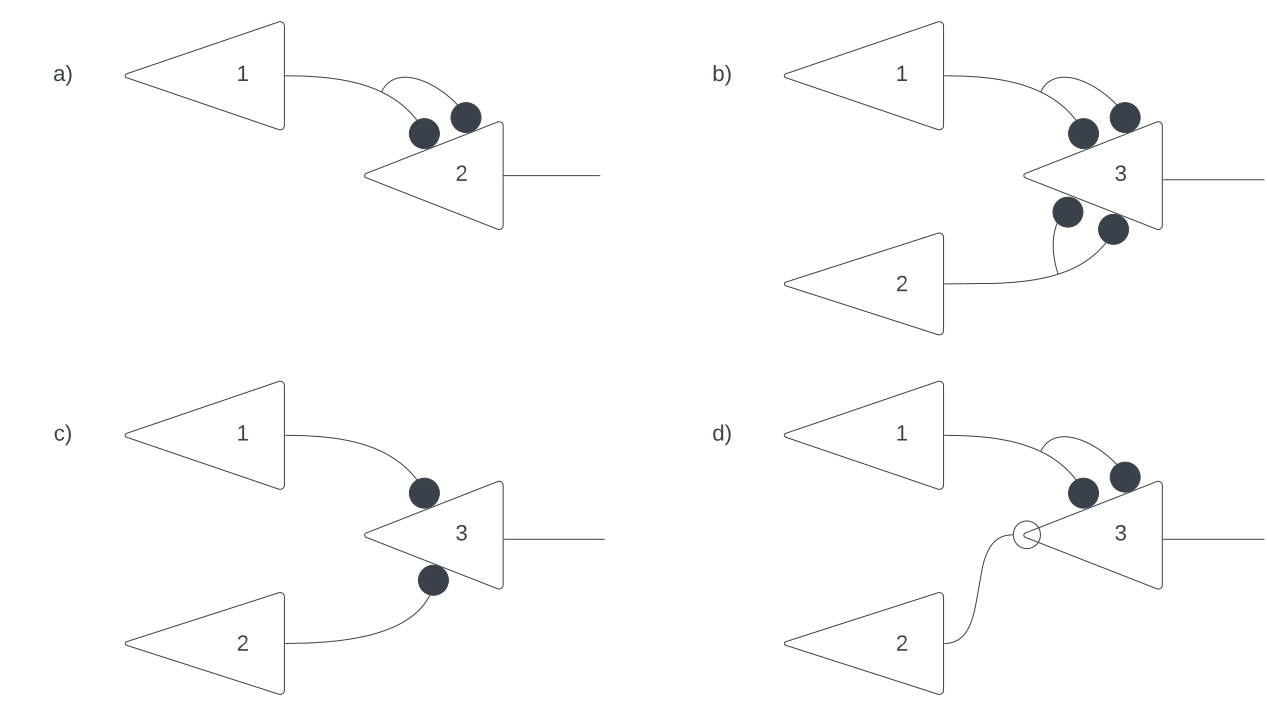
\includegraphics[
        width=16cm,
        keepaspectratio,
    ]{chapters/3. Kuenstliche Neuronen/images/mcpneuron}
    \caption{Schematische Darstellung von MCP-Zellen (Quelle: in Anlehnung an~\cite[105, Figure 1]{MP43})}
    \small
     Schwarze Kreise sind erregende Verbindungen, offene Kreise hemmende. Im ursprünglichen Modell benötigt ein Neuron zwei erregende Eingaben, um aktiviert zu werden.\\
    In a) ist damit ein Netz dargestellt von zwei Neuronen, bei denen $N_2$ feuert, wenn $N_1$ feuert. Unter Berücksichtigung der Zeiteinheit folgt die formale Darstellung $N_2(t) \equiv N_1(t - 1)$.\\
    Gleicherwiese ergibt sich für b), das $N_3$ nur feuert, wenn $N_1$ \textbf{oder} $N_2$ feuern: $N_3(t) \equiv N_1(t - 1) \lor N_2(t - 1)$.\\
    Analog folgt für c) $N_3(t) \equiv N_1(t - 1) \land N_2(t - 2)$.\\
    Für d) ergibt sich somit $N_3(t) \equiv N_1(t - 1 ) \land \neg N_2(t - 1)$
\end{figure}


\subsection{Aktivierungs- und Eingabefunktion}\label{mcp-inputactivfunc}

Mit $n \in  \mathbb{N}_0$ und $m \in  \mathbb{N}_0$ legen wir fest, dass ein Neuron $n + m$ Eingaben haben soll, mit $n \geq 1 \lor m \geq 1$, wobei $n$ die Anzahl der erregenden und $m$ die der hemmenden Eingaben ist.

Für die Schwellenwertfunktionen eines Neurons $N$ ergeben sich folgende Anforderungen: Die Summe der erregenden Eingabesignale $x_1, x_2, ..., x_n$ und der hemmenden Eingabesignale $y_1, y_2, ..., y_m$  muss den für das Neuron festgelegten Schwellenwert $\Theta \in  \mathbb{N}_0$ überschreiten, damit als Ausgabe eine $1$ erzeugt wird, ansonsten liefert die Funktion eine $0$ zurück.

\subsection*{Eingabefunktion}
Zur Integration der eingehenden Signale benötigen wir eine \textbf{Eingabefunktion}.
Der Wert dieser Eingabefunktion wird dann auf eine Funktion angewendet, die entscheidet, ob das Neuron feuert oder nicht - also eine $1$ oder $0$ ausgibt.\\

\noindent
Für die Eingabesignale $X$

\begin{equation}
X \in \{1, 0\}^{n+m} \coloneqq (x_1, x_2 ..., x_n, y_1, y_2, ... y_m)
\end{equation}\linebreak[2]

\noindent
definieren wir die \textit{Gewichte} $w_+ \in \{2, 1\}$ mit $w^1_+ \coloneqq1, w^2_+ \coloneqq 2$ für erregende Signale, $w_- \coloneqq -1$ für hemmende Signale (vgl.~\cite[27-28]{Fau94}).\\


\noindent
Die \textbf{Eingabefunktion} $g$

\begin{equation}
g: \{1, 0\}^{n+m} \to  \mathbb{Z}, X \mapsto \sum^n_{j=1} x_jw_+ + \sum^m_{k=1} y_kw_-
\label{eq:gl-mcpinpfunc}
\end{equation}\linebreak[2]

\noindent
liefert die Summe der hemmenden und erregenden Eingabesignale zurück.


\subsection*{Aktivierungsfunktion}
Die Schwellenwertfunktion wird im Kontext von künstlichen neuronalen Netzen auch \textbf{Aktivierungsfunktion} genannt (vgl. ~\cite[847]{RN09}), da sie entscheidet, ob einzelne Neuronen aktiviert werden oder nicht. In diesem Fall realisieren wir sie als \textbf{Treppenfunktion}\footnote{
    auch \textbf{Heaviside}-Funktion, die für beliebige negative Zahlen $0$ zurückliefert, ansonsten $1$. Wir werden später sehen, wie wir einen Schwellenwert wie in Gleichung~\ref{eq:gl-activation} in die Berechnung der Summe einfliessen lassen können, um die Funktion in dieser Form zu nutzen.
}, die $1$ zurückliefert, falls $g(X) >= \Theta$, und $0$ sonst :

\begin{equation}
f:  \mathbb{Z} \to \{0, 1\}, f(u) = f(g(X)) = \begin{cases}
                                          1  &\text{falls } u >= \Theta \\
                                          0 &\text{falls } u < \Theta
\end{cases}
\label{eq:gl-activation}
\end{equation}\linebreak[2]


\noindent
Da die Erregung absolut ist, muss $\Theta$ die Ungleichung

\begin{equation}
\Theta > (\sum^{k^{w_+^2}}_{j=1} 2) + (\sum^{k^{w_+^1}}_{j=1} 1) - w_-
\end{equation}\linebreak[2]



\noindent
erfüllen, was wir abkürzen können zu

\begin{equation}
\Theta > 2k^{w_+^2} + k^{w_+^1} - 1
\end{equation}


\subsection{McCulloch-Pitts-Netz als Graph}

Ein zyklenfreies Netz aus MCP-Zellen können wir wie folgt definieren (vgl.~\cite[32 ``Definition 2.1``]{Roj93}):


\begin{definition} Ein MCP-Netz ist ein gerichteter Graph\footnote{
    Gerichtete Kanten eine MCP-Netzes nehmen eigentlich keine Gewichtung der Information vor~\cite[40]{Roj93} (\textit{Rojas} verweist darauf, dass Gewichte in absolut hemmenden Leitungen unsinnig sind: Siehe~\cite[42]{Roj93}). Sowohl \textit{Minsky} in~\cite[34]{Min67} als auch \textit{Rojas} in~\cite[32]{Roj93} nutzen unter Berücksichtigung der \textit{absoluten Hemmung} nur die Summe der erregenden Signale und vergleichen diese mit $\Theta$ - dieser Vergleich findet nur statt, wenn \textit{kein} hemmendes Signal ankommt: Die Zelle liefert sonst direkt $0$ als Ausgabe zurück. \textit{Fausett} nutzt unter Berücksichtigung von Gleichung~\ref{eq:gl-activation} gewichtete Kanten, in ähnlicher Weise auch \textit{Beale und Jackson}~\cite[41]{BJ90}. \textit{Minsky} weist auf die Äquivalenz eines solchen Modells hin (vgl. ~\cite[34 f.]{Min67}), dessen wir uns im Folgenden auch bedienen werden.
} $G = (V, E)$ mit der Knotenmenge

\begin{equation}
V(G) =\{N_1, N_2, ... N_z\}
\end{equation}

und der paarweise verschiedenen Kantenmenge

\begin{equation}
E(G) = \{ (N^1_i, N_{i+1}), ..., (N^k_i, N_{i+1}) | i <= |V(G)|, k \in \mathbb{N} \}
\end{equation}

sowie der Kantengewichtsfunktion\footnote{
der Einfachheit halber wird bei der Fallunterscheidung keine weitere Unterteilung der für $w_+$ möglichen Werte $\{1, 2\}$ unternommen
}

\begin{equation}
\gamma: N^2 \to \{w_+, w_-\}, \gamma((N^k_i, N_{i+1})) = \begin{cases}
                                                              w_- \text{ falls } (N^k_i, N_{i+1})  \text{ hemmend } \\
                                                              w_+  \text{ sonst}
\end{cases}
\end{equation}
\label{def:mcpnetz}
\end{definition}



\subsection{Implementierung von Booleschen Funktionen}\label{seq-mcpbool}

Mit den eingeführten Formalismen können wir nun aussagenlogische Funktionen auf Basis von MCP-Zellen modellieren.


\subsection*{AND (Konjunktion)}
In der zweiwertigen Aussagenlogik liefert die \textbf{AND}-Funktion ($\land$) nur dann die Ausgabe ``wahr``, wenn die darin verknüpften Aussagen jeweils den Wahrheitswert ``wahr`` besitzen.

Für ``wahr`` = $1$ und ``falsch``= $0$ sieht die Wahrheitstabelle für zwei Aussagen wie folgt aus (Tabelle~\ref{tab:and}):

\setlength{\tabcolsep}{1.5em}
{\renewcommand{\arraystretch}{1.5}%
\begin{table} %[hbtp]
    \centering
    \begin{tabular}{c | c | c }
        \textbf{$A$} & \textbf{$B$} & \textbf{$A \land B$} \\
        \hline
        1  & 1 & 1 \\
        1  & 0 & 0 \\
        0  & 1 & 0 \\
        0  & 0 & 0 \\
    \end{tabular}
    \caption{Wahrheitstabelle für \textbf{AND}}
    \label{tab:and}
\end{table}



Wir legen für $N$ zwei erregende Eingabesignale $x_1, x_2$ sowie den Schwellenwert $\Theta = 2$ fest. Die Gewichte für $x_1$ und $x_2$ sind jeweils $w^1_+$ (s. Kantengewichtsfunktion in Definition~\ref{def:mcpnetz}).

Mit den oben eingeführten Definition verhält sich unser MCP-Neuron wie folgt (siehe Tabelle~\ref{tab:mcp-and}):

\begin{table} %[hbtp]
    \centering
    \begin{tabular}{c | c | c |c }
        $x_1w^1_+$ & $x_2w^1_+$ & $g_{and}(X)$ & $f_{and}(x)$ \\
        \hline
        1     & 1     & 2      &   1   \\
        1     & 0     & 1      &   0   \\
        0     & 1     & 1      &   0   \\
        0     & 0     & 0      &   0   \\
    \end{tabular}
    \caption{Werte der Aktivierungs- und Eingabefunktion für eine \textbf{AND-MCP-Zelle}}
    \label{tab:mcp-and}
\end{table}


\subsection*{OR (Disjunktion)}

Für die \textbf{OR}-Funktion ($\lor$) legen wir $\Theta = 2$ und zwei erregende Eingabesignale $x_1, x_2$ fest.
Die Gewichte für $x_1$ und $x_2$ sind jeweils $w^2_+$: Zusammen mit $\Theta = 2$ reicht also eine erregende Eingabe aus (siehe Tabelle~\ref{tab:mcp-or} sowie Abbildung~\ref{fig:mcpor}):


\begin{table} %[hbtp]
    \centering
    \begin{tabular}{c | c | c |c | c | c|c}
 $A$ & $B$ & $A \lor B$ & $x_1w^2_+$ & $x_2w^2_+$ & $g_{or}(X)$ & $f_{or}(x)$ \\
\hline
 1   & 1   & 1          & 2     & 2     & 4           & 1            \\
 1   & 0   & 0          & 2     & 0     & 2           & 1            \\
 0   & 1   & 0          & 0     & 2     & 2           & 1            \\
 0   & 0   & 0          & 0     & 0     & 0           & 0            \\
\end{tabular}
\caption{Werte der Aktivierungs- und Eingabefunktion für eine \textbf{OR-MCP-Zelle}}
\label{tab:mcp-or}
\end{table}


\begin{figure}[h]
    \centering
    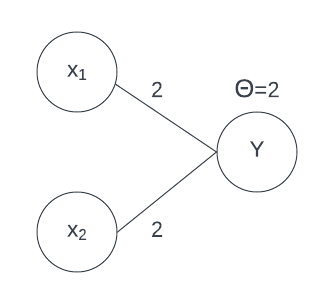
\includegraphics{chapters/3. Kuenstliche Neuronen/images/mcpor}
    \caption{Ein MCP-Neuron zur Modellierung von \textbf{OR} (Quelle: Eigene Darstellung)}
    \label{fig:mcpor}
\end{figure}


\subsection*{NOT (Negation)}

Für die \textbf{NOT}-Funktion ($\neg$) legen wir $\Theta = 0$ und ein erregendes Eingabesignal $x_1$ fest.
Das Gewicht für $x_1$ ist $w_-$: Zusammen mit $\Theta = 0$ würde also ein aktiv anliegendes Signal zu $1  w_-=-1 < \Theta = 0$.
Durch die resultierende Hemmung kann das Signal die Zelle nicht aktivieren (siehe Tabelle~\ref{tab:mcp-neg}):


\begin{table} %[hbtp]
    \centering
    \begin{tabular}{c | c | c |c | c | c}
        $A$ & $\neg A$ & $x_1$ & $g_{\neg}(X)$ & $f_{\neg}(x)$  \\
        \hline
         1   & 0        & -1     &  -1             & 0             \\
         0   & 1        & 0     &  0             &  1             \\
    \end{tabular}
    \caption{Werte der Aktivierungs- und Eingabefunktion für eine \textbf{NOT-MCP-Zelle}}
    \label{tab:mcp-neg}
\end{table}


\subsection*{NAND (NOT AND)}

$\{\neg, \lor, \land\}$ bilden ein vollständiges Operatorensystem, d.h., jede boolesche Funktion lässt sich durch einen aussagenlogischen Ausdruck  beschreiben, in dem ausschließlich Operatoren aus dieser Menge vorkommen (vgl.~\cite[89]{Hof22}).
Wie wir oben gesehen haben, können wir über MCP-Zellen die Operatoren $\neg, \lor, \land$ darstellen.
Ein MCP-Netz ist nach Definition also in der Lage, jede boolesche Funktion zu modellieren - wozu allerdings bereits $\{\neg, \land\}$ ausreicht, wie \textit{Sheffer} in~\cite{She13} zeigt.

$\{\neg, \land\}$ bildet die Operatorenmenge für \textbf{NAND}, was als MCP-Netz wie folgt modelliert werden kann (siehe Tabelle~\ref{tab:nand} sowie Abbildung~\ref{fig:mcpnand}):

\begin{table} %[hbtp]
    \centering
    \begin{tabular}{c | c | c}
        $A$ & $B$ & $\neg(A \land B)$ \\
        \hline
        1   & 1   & 0           \\
        1   & 0   & 1           \\
        0   & 1   & 1           \\
        0   & 0   & 1           \\
    \end{tabular}
    \caption{Die Wahrheitstabelle für \textbf{NAND}}
    \label{tab:nand}
\end{table}


Wir legen $\Theta_1 = 2$ fest (s. \textbf{AND}-Zelle), an dem zwei erregende Eingaben anliegen. $\Theta_2$ ist $0$ (s. \textbf{NOT}-Zelle) und besitzt eine hemmende Eingabe.

$N_1$ (\textbf{AND}) wird aktiviert, wenn sowohl $x_1$ als auch $x_2$ ein erregendes Signal weiterleiten. Das Ausgabesignal von $N_1$  wird dann ``invertiert`` (siehe Abbildung~\ref{fig:mcpnand}).


\begin{figure}[h]
    \centering
    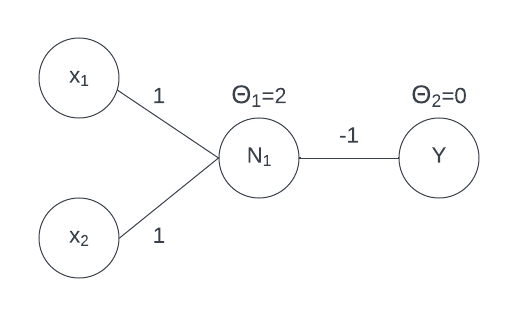
\includegraphics{chapters/3. Kuenstliche Neuronen/images/mcpnand}
    \caption{Ein MCP-Netz zur Modellierung von \textbf{NAND} (Quelle: Eigene Darstellung)}
    \label{fig:mcpnand}
\end{figure}


\subsection*{XOR (exclusive or)}

Eine weitere boolesche-Funktion, die aus mehreren MCP-Zellen als Netz modelliert werden kann, ist die \textbf{XOR}-Funktion (``exclusive or``). Die Wahrheitstabelle hierfür ist in Tabelle~\ref{tab:xor} zu finden.

\begin{table} %[hbtp]
    \centering
    \begin{tabular}{c | c | c}
        $A$ & $B$ & $A \oplus B$ \\
        \hline
        1   & 1   & 0           \\
        1   & 0   & 1           \\
        0   & 1   & 1           \\
        0   & 0   & 0           \\
    \end{tabular}
    \caption{Die Wahrheitstabelle für \textbf{XOR}}
    \label{tab:xor}
\end{table}


Für die Konstruktion des Netzes rufen wir uns Abbildung~\ref{fig:mcpor} ins Gedächtnis. $\Theta = 2$ wird übertroffen, wenn entweder $x_1$ oder $x_2$ ein erregendes Signal weiterleitet. Allerdings wird $\Theta$ auch übertroffen, wenn jeweils $x_1$ \textit{und} $x_2$ gleichzeitig aktiv sind, denn dann ist $f_{xor}(g(X)) = 4$.
Also muss eine Hemmung zwischengeschaltet werden (s. Abbildung~\ref{fig-mcpxorf}): Ein aktives $x_1$ hemmt $N_2$. $N_2$ leitet in dem Fall $0$ an $Y$ weiter. Die Zellen $x_2$ und $N_1$ werden analog verbunden.

Die \textbf{disjunktive Normalform} (Gleichung~\ref{eq:gl-xordis}) und die \textbf{konjunktive Normalform} (Gleichung~\ref{eq:gl-xorcon}) von \textbf{XOR} liefern die Formel für das Netz, wobei insb. die disjunktive Normalform die abgebildete Verschaltung in Abbildung~\ref{fig-mcpxorf} erklärt.\\

\begin{equation}
A \oplus B \equiv (\neg A \land B) \lor (A \land \neg B)
\label{eq:gl-xordis}
\end{equation}

\begin{equation}
A \oplus B \equiv (A \lor B) \land (\neg A \lor \neg B)
\label{eq:gl-xorcon}
\end{equation}


\begin{figure}[h]
    \centering
    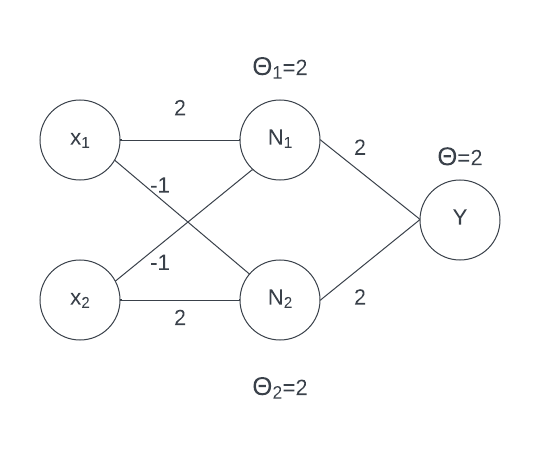
\includegraphics{chapters/3. Kuenstliche Neuronen/images/mcpxor}
    \caption{Entwurf für ein MCP-Netz zur Modellierung von \textbf{XOR}}
    \label{fig-mcpxorf}
\end{figure}


Für weitere Beispiele zu Modellierungen von MCP-Netzen sei auf Anhang~\ref{appendix:paradoxehitzeempfindung} verwiesen.








